\documentclass[11pt]{amsart}
\usepackage[margin=1.15in]{geometry}
\usepackage{amssymb,amsmath,booktabs,enumitem,xcolor,graphicx,tikz,array}
\usepackage{standalone}
\usepackage{float}
\usepackage[colorlinks,linkcolor=blue!50!black,urlcolor=blue!50!black,citecolor=blue!50!black]{hyperref}

\newcommand{\ch}{\operatorname{ch}}
\newcommand{\Hom}{\operatorname{Hom}}
\newcommand{\RP}{\mathbb{RP}^2}
\newcommand{\Z}{\mathbb{Z}}
\newcommand{\lab}[1]{\texttt{#1}}
\newcommand{\file}[1]{\texttt{#1}}
\newcommand{\inv}{^{-1}}

\theoremstyle{plain}
\newtheorem{fact}{Statement}
\theoremstyle{remark}
\newtheorem*{caveat}{Caveat}

\definecolor{sk}{RGB}{30,58,138}
\tikzset{strand/.style={sk,line width=1.1pt,line cap=round}, marker/.style={black,line width=2.6pt,line cap=round}}

\title[A machine census of surface-links by ch-index]{A machine census of surface-links by ch-index:\\
what was computed, what it proves, and what it does not}
\date{15 November 2026. Describes the audit of commit \texttt{3089bb0}, the subsequent post-audit remediation
and verification of the repository, and the completed ch-index $12$ census. Evidence and scripts are in
\file{AUDIT.md} and \file{audit\_scripts/}.}

\begin{document}

\begin{abstract}
The \texttt{surfaceknots} repository enumerates marked graph diagrams of closed surfaces in $\mathbb{R}^4$
and sorts them with a battery of invariants, extending Yoshikawa's 1994 table of surface-links from
ch-index~$10$ through ch-index~$12$. This note states what the computation establishes and with what degree
of certainty. Run blind, the pipeline recovers every class of Yoshikawa's table at ch-index $9$ and~$10$.
At ch-index~$11$ it finds ten weakly prime invariant classes (nine singletons and one three-diagram packet)
and leaves $93$ diagrams unresolved; at ch-index~$12$, after fixing the invariant and pruning defects found
at commit \texttt{3089bb0} (Sections~\ref{sec:evidence}--\ref{sec:corrections}), the full census across all
saddle strata finds $34$ weakly prime invariant classes ($20$ singletons and $14$ packets, on $63$ diagrams)
and leaves $742$ diagrams unresolved. Four structural results stand out. First, the group of the
ch-index-$11$ Klein bottle \lab{11\_1\^{}-2} is the binary octahedral group of order~$48$. Second, seventeen
of the $33$ entries through ch-index~$11$ are two or three unknotted spheres with a single $1$-handle named
by a free-group cord word $w$ (Table~\ref{tab:names}); while $\ch(K(w))=\ch(T(w))+1$ holds on six small words
(predicting $K(baba\inv b\inv)$ and $K(bab\inv ab)$ at $\ch=12$), the cord $w=bab\inv a\inv b$ refutes
universal equality with $\ch(K(w))=11<12=\ch(T(w))$. Third, $1$-handle double cosets settle unresolved
diagrams by exact calculation where bounded move search fails. Fourth, two twelve-vertex $2$-knots
(\lab{12\_10} and \lab{12\_8}) are proved to have Cappell--Shaneson groups $\Z^3\rtimes_{A_i}\Z$
(Statement~\ref{st:cs}), determining their punctured-$T^3$-fibered exteriors topologically up to Gluck twist.
\end{abstract}

\maketitle

\section{The objects}

A \emph{surface-link} is a closed surface $F$, possibly disconnected and possibly non-orientable, smoothly
embedded in $\mathbb{R}^4$. Two are the same if an isotopy of $\mathbb{R}^4$ carries one to the other; in
this project mirror images are also identified. A connected surface-link is a \emph{surface-knot}; a
knotted sphere is a \emph{$2$-knot}.

Slice $\mathbb{R}^4$ by a time coordinate $t$. Each slice of $F$ is a link in $\mathbb{R}^3$, and as $t$
increases the link changes in three ways: a small circle is born (a minimum of $t$ on $F$), a small circle
dies (a maximum), or two strands merge and reconnect (a saddle). Every surface-link can be moved so that
all its minima lie below $t=0$, all its maxima above, and all its saddles exactly at $t=0$. The slice at
$t=0$ is then a link diagram in which each saddle appears as a four-valent vertex carrying a short bar,
the \emph{marker}. Such a picture is a \emph{marked graph diagram} or \emph{ch-diagram}.

\begin{figure}[ht]
\centering
\begin{tikzpicture}[scale=0.8]
  \begin{scope}
    \draw[strand] (-1,-1)--(1,1); \draw[strand] (-1,1)--(1,-1);
    \draw[marker] (-0.45,0)--(0.45,0);
    \node[below] at (0,-1.15) {marked vertex};
  \end{scope}
  \begin{scope}[xshift=4.2cm]
    \draw[strand] (-1,1) .. controls (-0.25,0.25) and (0.25,0.25) .. (1,1);
    \draw[strand] (-1,-1) .. controls (-0.25,-0.25) and (0.25,-0.25) .. (1,-1);
    \node[below] at (0,-1.15) {$L_+$: just above $t=0$};
  \end{scope}
  \begin{scope}[xshift=-4.2cm]
    \draw[strand] (-1,1) .. controls (-0.25,0.25) and (-0.25,-0.25) .. (-1,-1);
    \draw[strand] (1,1) .. controls (0.25,0.25) and (0.25,-0.25) .. (1,-1);
    \draw[black!45,line width=0.8pt,dashed] (-0.42,0)--(0.42,0);
    \node[below] at (0,-1.15) {$L_-$: just below $t=0$};
  \end{scope}
  \draw[->,black!50] (-2.7,0)--(-1.6,0); \draw[->,black!50] (1.6,0)--(2.7,0);
\end{tikzpicture}
\caption{A saddle. Below $t=0$ two strands approach along the dashed line; at $t=0$ they touch, which is
drawn as a vertex with a marker; above $t=0$ they have reconnected. Smoothing every marked vertex one way
gives the link $L_-$, the other way $L_+$.}
\label{fig:vertex}
\end{figure}

Smoothing all marked vertices as in Figure~\ref{fig:vertex} gives two classical links, $L_-$ just below
$t=0$ and $L_+$ just above. The diagram describes a closed surface exactly when both are unlinks, because
only then can the slices below and above be capped off by disks. Such a diagram is called
\emph{admissible}. Figure~\ref{fig:movie} shows an example. The Euler characteristic of the surface is
the number of circles of $L_-$, plus the number of circles of $L_+$, minus the number of marked vertices.

\begin{figure}[ht]
\centering
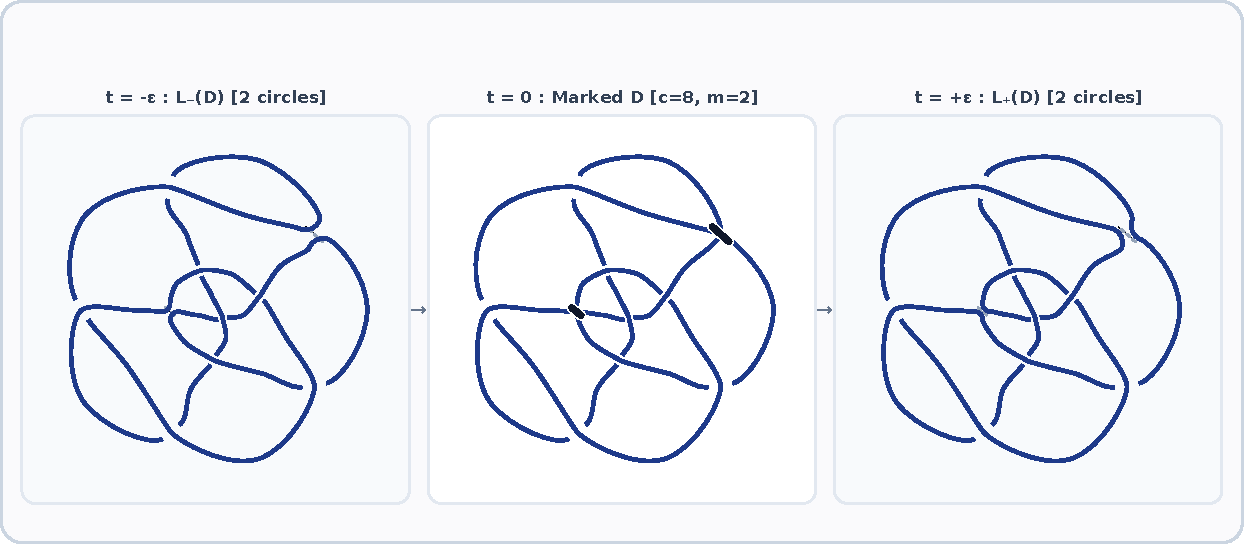
\includegraphics[width=0.98\textwidth]{fig_10_2_movie.pdf}
\caption{The entry \lab{10\_2} of Yoshikawa's table, the $2$-twist-spun trefoil. Centre: its ch-diagram,
with eight crossings and two marked vertices. Left and right: $L_-$ and $L_+$, each a two-component
unlink. Two minima, two saddles and two maxima give a sphere. (Figure generated by the repository.)}
\label{fig:movie}
\end{figure}

Two admissible diagrams represent the same surface-link if and only if they differ by a sequence of eight
local moves, the \emph{Yoshikawa moves} $\Omega_1,\dots,\Omega_8$ (Swenton; Kearton--Kurlin). The first
three are the Reidemeister moves; the others slide strands over markers, create or cancel a marked vertex
together with a trivial circle, and exchange pairs of markers.

The \emph{ch-index} of a diagram is its number of vertices, crossings plus markers. The ch-index $\ch(F)$
of a surface-link is the least ch-index of any diagram of it. Yoshikawa~\cite{Y} listed the $23$
surface-links with $\ch\le 10$ that are \emph{weakly prime}: not a connected sum $F_1\# F_2$ with
$\ch(F_1)<\ch(F)$ and $\ch(F_2)<\ch(F)$. Every surface-link is a connected sum of weakly prime ones of
ch-index at most its own, so the table generates everything with $\ch\le 10$. Weak primeness is weaker than
primeness: the standard projective plane $P$ is in the table although $P = F\# P$ for a knotted sphere
$F$ of ch-index $10$.

The labels follow Yoshikawa's convention. \lab{10\_2\^{}0,-2} is the second entry with $\ch=10$ whose
components are a sphere (symbol $0$) and a Klein bottle (symbol $-2$). A positive symbol is the genus of
an orientable component; a negative symbol counts projective-plane summands of a non-orientable one, so
$-1$ is $\RP$ and $-2$ is the Klein bottle. A label with no superscript is a $2$-knot.

\section{The computation}\label{sec:pipeline}

The pipeline has five stages. Each is described with the property it needs in order for the final list
to be trustworthy.

\begin{enumerate}[leftmargin=*]
\item \textbf{Shadows.} Forgetting crossing and marker information leaves a four-valent graph on the
sphere. Only graphs without a two-edge cut are needed: a diagram whose graph has such a cut is a
connected sum of two smaller diagrams. These graphs are dual to simple quadrangulations of the sphere and
are counted by OEIS A113201: $803$ with ten vertices, $3{,}378$ with eleven, $15{,}882$ with twelve.
\emph{Needed: the list is complete.}

\item \textbf{Vertex assignments.} Each vertex is made one of two crossings or one of two markers, giving
$4^n$ candidates per shadow, about $1.4\times 10^{10}$ at $n=11$. Candidates are discarded when a cheap
necessary condition for admissibility fails (the Kauffman bracket of $L_\pm$ must be that of an unlink) or
when an obvious simplifying move applies. \emph{Needed: nothing admissible and irreducible is discarded.}

\item \textbf{Admissibility.} For each survivor, explicit Reidemeister sequences reducing $L_+$ and $L_-$
to crossingless diagrams are found. \emph{Needed: every reported sequence is valid; a failure to find one
does not silently remove a diagram that matters.}

\item \textbf{Moves.} Diagrams are merged when Yoshikawa moves connect them and discarded when moves reach
a diagram with fewer vertices. Because a simplification may need to pass through larger diagrams first,
the search is allowed to add one or two vertices before coming back down. It is a bounded search.
\emph{Needed: every implemented move is a genuine isotopy.} Completeness of the search is \emph{not}
needed for correctness; it only affects how many diagrams are left over.

\item \textbf{Invariants.} Each surviving diagram receives a key built from ten layers of invariants: the
topology and normal Euler numbers of the components; the first homology of the complement; Alexander
ideals; the double branched cover; homology of finite covers; counts of homomorphisms from the group to
ten finite groups; kei and biquandle colouring modules; quandle cocycle state sums; linking invariants;
and a count of peripheral representations. Survivors with different keys are meant to be different
surfaces. \emph{Needed: each layer is an isotopy invariant and the comparison of values never reports a
difference that is not there.}
\end{enumerate}

\section{What an entry of the census means}\label{sec:meaning}

Suppose the moves and invariants are sound. Fix $N$, run the pipeline on all shadows with $N$ vertices,
and let $D$ be a surviving diagram whose invariant key $k$ matches no surface of smaller ch-index and no
connected sum of two surfaces of smaller ch-index.

\begin{fact}\label{st:new}
The surface of $D$ has ch-index exactly $N$. If $D$ is the only survivor with key $k$, then it is the
only surface-link with $\ch\le N$ and key $k$.
\end{fact}

The reason is short. A diagram with $N$ vertices of a surface with key $k$ either has a two-edge cut,
or is discarded because moves reduce it, or is merged into a survivor by moves, or survives. The second
puts the surface below ch-index $N$, where key $k$ does not occur. The first makes it a connected sum of
two surfaces of smaller ch-index, which the hypothesis excludes. For the classes of
Section~\ref{sec:eleven} that hypothesis is the check of Section~\ref{sec:weak}; for two of them it needs
the knot types of the components in addition to the key.

Three limits on Statement~\ref{st:new} matter in practice.

\begin{itemize}[leftmargin=*]
\item \emph{It needs the list of keys below $N$.} For $N=11$ that list comes from Yoshikawa's table,
which was compiled by hand. Section~\ref{sec:blind} reports a blind re-run that supports it.
\item \emph{Several survivors with one key are not known to be one surface.} The search is bounded, so two
diagrams of the same surface can both survive. The repository calls such a group a \emph{packet}.
\item \emph{A survivor whose key does occur below $N$ is unresolved.} It is either an awkward diagram of a
known surface or a new surface that the invariants cannot tell from a known one. The repository calls
these \emph{ambiguous}.
\end{itemize}

The second hypothesis of Statement~\ref{st:new} implies that the surface is weakly prime.
The statement says nothing about primeness in the strict sense, where a summand may have any ch-index;
Section~\ref{sec:corrections} returns to this.

To keep epistemic boundaries explicit, every claim in the census and family catalogue falls into one of five
degrees of certainty:
\begin{enumerate}[leftmargin=*]
\item \emph{Constructively / move-certified} (\lab{MOVE\_CERTIFIED}): explicit admissible ch-diagrams whose
smoothings $L_\pm$ carry verified $\mathrm{R1}$--$\mathrm{R3}$ unlinking movies, and explicit local
$\Omega_1$--$\Omega_8$ / 4D flype paths certifying unoriented isotopy in $\mathbb{R}^4$ (up to ambient
$\mathrm{O}(4)$).
\item \emph{Algebraically proved}: presentation-independent invariants of $\pi_1(S^4\setminus F)$ proved by
finite confluent Knuth--Bendix rewriting, coset enumeration, meridian-pinned strong Gr\"obner bases for
$E_k\subset\Z[H_1]$, finite-index regular cover homology, or group deficiency obstructions
($\operatorname{def}(\pi_1)\le 0\implies$ non-ribbon).
\item \emph{Census-exact modulo lower-$\ch$ completeness}: for \lab{EXACT\_SINGLETON} and \lab{NEW\_PACKET}
entries, exhaustion over 2-edge-cut-free shadows (OEIS A113201) together with disjunction from all
lower-$\ch$, unknot, split, and weakly reducible connected-sum cells proves $\ch(F)=N$ conditional on
completeness of the table below $N$. Inside a \lab{NEW\_PACKET}, the invariant cell attains $\ch=N$, whereas
merging all packet members into a single smooth surface remains open until move-connected.
\item \emph{Topologically vs.\ smoothly identified}: 4-manifold fibration and surgery theorems (Hillman~\cite{Hil}
for Cappell--Shaneson groups $\Z^3\rtimes_{A_i}\Z$; Conway--Orson--Powell for $\pi_1\cong\Z_2$ projective
planes) determine the topological embedding or exterior (up to non-reflexive Gluck twist
$\epsilon\in\{0,1\}$ in the Cappell--Shaneson case), whereas pinning down the smooth isotopy framing
requires 2-/3-handle Kirby calculus beyond $\pi_1$.
\item \emph{Heuristic invariant match or unresolved} (\lab{INVARIANT\_MATCH} / \lab{AMBIGUOUS\_SHADOW}):
matching a compiled model of ch-index $>N$ to a census cell solely by 10-layer invariant agreement without a
move path, or leaving a survivor unresolved because its key already appears below $N$.
\end{enumerate}

\section{Results}

\subsection{Blind recovery of the known table}\label{sec:blind}

The repository's dataset for $\ch\le 10$ is built from $23$ diagrams entered by hand. As a test of the
pipeline we ran it with no input at $N=9$ and $N=10$, over all topological types, and computed
homomorphism counts for every survivor.

\begin{center}
\begin{tabular}{@{}lrrl@{}}
\toprule
$N$ & shadows & survivors & of which \\
\midrule
$9$ & $198$ & $12$ & the $3$ table classes, one diagram each; $9$ with cyclic group \\
$10$ & $803$ & $54$ & the $12$ table classes on $17$ diagrams; $36$ with cyclic group; $1$ other \\
\bottomrule
\end{tabular}
\end{center}

Every class of Yoshikawa's table with ch-index $9$ or $10$ appears, and no survivor has a non-cyclic
group that is absent from the table. The survivors with cyclic group are diagrams with the invariants of
an unknotted surface that the bounded search does not reduce; $25$ of the $45$ are removed by a rule based
on a theorem about $1$-handles (Section~\ref{sec:handles}), and $20$ remain. The one other survivor is a
sphere--torus link with the invariants of \lab{6\_1\^{}0,1}.

Two lessons follow. First, the pipeline and the table agree, which is evidence for both. Second, the
search does not merge all diagrams of a class even where the answer is known: \lab{10\_1}, \lab{10\_2}
and \lab{10\_3} each survive as two diagrams and \lab{10\_1\^{}1} as three. Packets and unresolved
diagrams are therefore the normal output of this search and are not, in themselves, a sign of new
surfaces.

\subsection{Ch-index 11}\label{sec:eleven}

According to the repository's stored dataset, of $3{,}378$ shadows $105$ diagrams survive.
A clean re-run of the whole pipeline from the committed code, made for this note, reproduces this: $105$ survivors, the same ten classes, and the same breakdown of the rest. (Two early counters in the repository's funnel table are stale: the scan leaves $66{,}017{,}754$ candidates, not $75{,}125{,}028$.)
Twelve of them carry ten keys that do not occur for $\ch\le 10$ (Table~\ref{tab:11},
Figure~\ref{fig:gallery}); by Statement~\ref{st:new} these are ten surface-links of ch-index exactly $11$,
nine of them the unique surface with their key at $\ch\le 11$. The remaining $93$ diagrams are
unresolved: $80$ have the invariants of a standard unknotted surface ($15$ of them of the unknotted
sphere, torus or projective plane of the table, $65$ of surfaces of higher genus), $4$ of a knotted table
entry, $8$ of a connected sum, and $1$ of a split union.

\begin{table}[ht]
\centering
\small
\begin{tabular}{@{}lp{0.14\textwidth}p{0.3\textwidth}p{0.34\textwidth}@{}}
\toprule
Label & Components & Group of the complement & What it is \\
\midrule
\lab{11\_1} & $S^2$ & one relator, $\Delta=2x^2-2x+1$ & ribbon, Yasuda's $Y3_4$; a packet of $3$ diagrams, read as $R(bab\inv a\inv)$ and $R(bab\inv a)$ \\
\lab{11\_2} & $S^2$ & one relator, $\Delta=x^3-x^2+2x-1$ & ribbon, $R(baba\inv)$ \\
\lab{11\_1\^{}-2} & Klein bottle, $e=0$ & binary octahedral, order $48$ & spun trefoil plus a non-orientable handle \\
\lab{11\_1\^{}0,1} & $S^2\sqcup T^2$ & one relator & $T(baba\inv b\inv)$ \\
\lab{11\_2\^{}0,1} & $S^2\sqcup T^2$ & one relator & $T(bab\inv ab)$ \\
\lab{11\_1\^{}0,-2} & $S^2\sqcup K^2$ & one relator & $K(bab\inv a\inv b)$ \\
\lab{11\_2\^{}0,-2} & $S^2\sqcup K^2$ & $\langle a,b \mid b^{2}ab^{-2}=a^{-1}\rangle$ & $K(b^2)$ \\
\lab{11\_3\^{}0,-2} & $S^2\sqcup K^2$ & one relator & $K(bab)$ \\
\lab{11\_1\^{}1,-2} & $T^2\sqcup K^2$ & $\Z_4\rtimes\Z$ & $T(bab\inv)$ with a second, twisted tube on $B$ \\
\lab{11\_1\^{}0,0,-2} & $S^2\sqcup S^2\sqcup K^2$ & $\cong$ group of a split link & three spheres, one twisted tube with cord $bc$ \\
\bottomrule
\end{tabular}
\caption{The ten keys first seen at ch-index $11$. The names $R(w)$, $T(w)$, $K(w)$ are explained in
Section~\ref{sec:names}.}
\label{tab:11}
\end{table}

\begin{figure}[ht]
\centering
\newcommand{\gal}[2]{\begin{minipage}[t]{0.19\textwidth}\centering
  \includestandalone[width=\linewidth]{../pics/tikz/#1}\\[-2pt]{\scriptsize\lab{#2}}\end{minipage}}
\gal{11_1}{11\_1}\hfill\gal{11_2}{11\_2}\hfill\gal{11_1_sup_m2}{11\_1\^{}-2}\hfill
\gal{11_1_sup_0_1}{11\_1\^{}0,1}\hfill\gal{11_2_sup_0_1}{11\_2\^{}0,1}\\[8pt]
\gal{11_1_sup_0_m2}{11\_1\^{}0,-2}\hfill\gal{11_2_sup_0_m2}{11\_2\^{}0,-2}\hfill
\gal{11_3_sup_0_m2}{11\_3\^{}0,-2}\hfill\gal{11_1_sup_1_m2}{11\_1\^{}1,-2}\hfill
\gal{11_1_sup_0_0_m2}{11\_1\^{}0,0,-2}
\caption{Diagrams of the ten classes of Table~\ref{tab:11}, as drawn by the repository. Colours mark
components; black bars are markers.}
\label{fig:gallery}
\end{figure}

No enumeration at ch-index $11$ appears in the literature that we could find. The $2$-knots in the table
are ribbon knots of a kind already classified by other means (Section~\ref{sec:names}); what the
census adds for them is the value of the ch-index.

\subsection{Are the ten classes weakly prime?}\label{sec:weak}

A class of ch-index $11$ is weakly prime if it is not a connected sum of two surfaces of ch-index at most
$10$. There are finitely many of those, so this can be checked. At commit \texttt{3089bb0} the repository
compared only with sums whose summands had total ch-index at most $12$, which is not enough because the
ch-index of a sum can drop far below the sum of its parts: $\ch(\lab{10\_3}\#P)=2$. We completed the check
independently (and the post-audit revision now synthesises unfiltered connected sums across all lower-$\ch$
entries in both \file{ch11\_census.py} and \file{ch12\_census.py}):

\begin{itemize}[leftmargin=*]
\item \lab{11\_1}, \lab{11\_2}. The first Alexander ideal of a sum is the product of those of the
summands. The polynomials $2x^2-2x+1$ and $x^3-x^2+2x-1$ are irreducible, differ from the Alexander
polynomials of \lab{8\_1}, \lab{9\_1}, \lab{10\_1}, and do not lie in the ideals $(x+1,3)$ and
$(x^2+x+1,2)$ of \lab{10\_2} and \lab{10\_3}.
\item \lab{11\_1\^{}-2}. Its meridian has order eight (Section~\ref{sec:new}).
\item The links. For each we formed every sum of two surfaces of ch-index at most $10$ with the right
components, $458$ sums in all, and compared homomorphism counts into seven finite groups. For five of
the seven links no sum agrees, or no sum exists.
\end{itemize}

The remaining two are instructive. \lab{11\_2\^{}0,1} has the same counts as
$\lab{6\_1\^{}0,1}\#\lab{8\_1}$, and \lab{11\_1\^{}0,-2} the same as
$\lab{7\_1\^{}0,-2}\#\lab{8\_1}$. These sums have summands of total ch-index $14$ and $15$, so the
repository never compared with them. The agreement is not an accident: the groups are isomorphic, and so
are the Alexander ideals. The surfaces are nevertheless different. In the sum, one component is knotted
(it contains the spun trefoil), while each component of the census link is unknotted. So all ten classes
are weakly prime, but for these two the proof is about components and not about the group of the link.
(Among the layers of the repository's key, the homology of finite covers also separates them from the sums.)

\subsection{Ch-index 12: full census and Cappell--Shaneson $2$-knots}\label{sec:twelve}

At commit \texttt{3089bb0} only two slices of ch-index $12$ had been inspected ($S^2$ with $m=2$, and $\RP$
with $m=3$), and coarse Alexander fingerprints together with missing regular-cover layers merged distinct
$2$-knots into single cells (hiding an $E_1=(3,x^2+1)$ packet inside the unknot cell and merging two
Cappell--Shaneson $2$-knots into ribbon cells). After remediating all ten invariant layers
(Section~\ref{sec:evidence}) and running the full C99/OpenMP pipeline across every saddle count
$m\in\{1,\dots,11\}$ on all $15{,}882$ prime shadows ($2.66\times 10^{11}$ raw assignments, $1.16\times 10^9$
bracket-filtered), $909$ raw post-tube diagrams and $805$ post-flype/mountain-pass diagrams survive. Sorting
them against all $\ch\le 11$ classes, unknots, split unions, and unfiltered connected sums yields
\textbf{$34$ weakly prime invariant classes} on $63$ diagrams ($20$ \lab{EXACT\_SINGLETON} and $14$
\lab{NEW\_PACKET}), leaving $742$ unresolved diagrams across $55$ \lab{AMBIGUOUS\_SHADOW} cells. Every
surviving $\RP$ diagram through $\ch\le 12$ has meridian order two, so the irreducible projective plane
of~\cite{HKMN} satisfies $\ch\ge 13$.

\paragraph{Why tabulate by $\ch$-index, and why the exhaustive census stops at $\ch=12$.}
Alternative four-dimensional complexity invariants fail to define finite census strata on their own:
triple-point number assigns zero to \emph{every} Artin-spun knot $\tau^0(K)$ (leaving infinitely many distinct
$2$-knots at complexity zero), while Meier--Zupan's tri-plane bridge index $b$ yields only unknotted surfaces
for $b\le 3$ and already admits infinitely many distinct $2$-knots at $b=4$ unless braid word length is bounded
simultaneously. By contrast, Yoshikawa's $\ch(F)=\min_D(c+m)$ counts all $4$-valent vertices of a planar marked
diagram, making $\ch(F)\le N$ manifestly finite at every $N$ and treating orientable, non-orientable, and
multi-component surface-links uniformly.
Computationally, each step $n\mapsto n+1$ multiplies the prime $4$-regular planar shadow count (\texttt{OEIS A113201}: $803$ at
$n=10$, $3{,}378$ at $n=11$, $15{,}882$ at $n=12$, $77{,}185$ at $n=13$) by $\approx 4.7$--$4.9\times$ while
multiplying the $4^n$ crossing/marker state space per shadow by $4\times$, creating an $\approx 19\times$
wall per vertex: $8.42\times 10^8$ raw states at $\ch=10$ ($1.6\,\mathrm{s}$ on $64$ cores),
$1.42\times 10^{10}$ at $\ch=11$ ($5.6\,\mathrm{min}$), $2.66\times 10^{11}$ at $\ch=12$ ($88.7\,\mathrm{min}$),
and $5.18\times 10^{12}$ at $\ch=13$ ($\sim 25$--$28\,\mathrm{h}$ across all $m\in\{1,\dots,12\}$, where $+2$
mountain-pass stabilization also reaches $n=15$). However, at fixed $\ch=n$, a slice with $m$ saddles inspects
only $\binom{n}{m}2^{n}$ states per shadow: at $\ch=12$, the middle sectors $m\in\{5,6,7\}$ consume $65\%$ of
the total runtime ($3{,}130\,\mathrm{s}$ of $4{,}846\,\mathrm{s}$), whereas the $m=2$ $2$-sphere slice takes
only $41.1\,\mathrm{s}$---making targeted low-saddle probes at $\ch=13$ (such as the $m=2$ $S^2$-sector)
feasible in minutes even where full $m=1\dots 12$ exhaustion requires a day of $64$-core compute.

Eleven of the $34$ classes at $\ch=12$ are connected $2$-knots (\lab{12\_1}--\lab{12\_11}). Beyond the
move-certified Artin spins \lab{12\_1} $=\tau^0(5_2)$ and \lab{12\_11} $=\tau^0(5_1)$, the determinant-$7$
$2$-twist-spin \lab{12\_6} ($\tau^2(5_2)$, $E_1=(7,x+1)$), and the ribbon singleton \lab{12\_3}
($\Delta=3t^2-3t+1$), three separations require the deeper invariant layers:
\begin{itemize}[leftmargin=*]
\item \textbf{Non-principal $\mathbb{F}_9$ ideal (\lab{12\_2}, packet of $2$ diagrams)}: strong Gr\"obner
bases isolate $E_1=(3,x^2+1)$ ($\Z[x^{\pm 1}]/E_1\cong\mathbb{F}_9$), so $\operatorname{def}(\pi_1)\le 0$
and \lab{12\_2} is strictly non-ribbon. Its group $\langle a,p\mid p^3,\, apa=papap\rangle$ has quotient
$|G/\langle\!\langle a^6\rangle\!\rangle|=720$ containing $\mathrm{SL}(2,5)$ (non-soluble), and the orders of
$G/\langle\!\langle a^k\rangle\!\rangle$ exclude all $k$-twist-spins $\tau^k(K)$ for $2\le k\le 7$.
\item \textbf{Mochizuki $R_5$ cocycle split (\lab{12\_4} vs.\ \lab{12\_5})}: both classes have
$E_1=(5,x+1)$, $\pi_1\cong\Z_5\rtimes_{-1}\Z$, and $25$ colourings by the dihedral quandle $R_5$; Mochizuki's
$3$-cocycle state sums ($5+10u^2+10u^3$ on the $5$-diagram packet \lab{12\_4} vs.\ $5+10u+10u^4$ on the
singleton \lab{12\_5}) separate $\tau^2(4_1)$ from $\tau^2(5_1)$.
\end{itemize}

The most striking objects in the census are two singletons in the $(c,m)=(10,2)$ $S^2$-stratum. The first,
\lab{12\_10} (\lab{CS\_A0}), is
\begin{center}\scriptsize
\texttt{X[1,2,3,4], X[5,6,4,7], X[6,8,9,1], Y[9,10,11,2], X[12,13,14,3], Y[14,15,16,7],}\\
\texttt{X[5,17,18,8], X[17,19,10,18], X[11,20,21,12], X[13,21,22,15], X[23,24,19,16], X[24,23,22,20]}
\end{center}
a sphere with two minima, two saddles and two maxima. It shares the Alexander polynomial $t^3-t^2+2t-1$ of
the $\ch=11$ ribbon knot \lab{11\_2}, and at commit \texttt{3089bb0} had been filed as a diagram of
\lab{11\_2}. Killing the cube of a meridian leaves the Frobenius group $F_{21}$ of order $21$, against order
$168$ for \lab{11\_2}; correspondingly, the $F_{21}$-regular cover has first homology $\Z\oplus\Z_7$ on
\lab{12\_10} versus $\Z\oplus\Z_2^5\oplus\Z_{14}$ on \lab{11\_2}. Its commutator subgroup is free abelian of
rank three:

\begin{fact}\label{st:cs}
The group of the complement of \lab{12\_10} is $\Z\ltimes_{A_0}\Z^3$, where $A_0\in\mathrm{SL}_3(\Z)$ has
characteristic polynomial $\det(tI-A_0)=t^3-2t^2+t-1$ (reciprocal $t^3-t^2+2t-1$ under meridian inversion).
\end{fact}

The proof is both a finite confluent Knuth--Bendix completion in GAP (giving normal forms $x^k u^a v^b w^c$
with commuting $u,v,w$, verified from two independent diagram presentations) and a hand derivation.
Running the same check on the $(10,2)$ $S^2$-stratum finds one further metabelian $\Z\ltimes\Z^3$
singleton, \lab{12\_8} (\lab{CS\_A1}):
\begin{center}\scriptsize
\texttt{X[1,2,3,4], X[4,5,6,1], X[7,8,9,6], Y[9,10,11,2], X[3,12,13,14], Y[14,15,16,17],}\\
\texttt{X[18,7,5,17], X[8,18,19,10], X[20,21,12,11], X[21,22,15,13], X[23,24,19,16], X[24,23,22,20]}
\end{center}
whose group is $\Z\ltimes_{A_1}\Z^3$ with $\det(tI-A_1)=t^3-3t^2+2t-1$ (reciprocal $t^3-2t^2+3t-1$). Its
$F_{57}$-regular cover has torsion $\Z_{19}$, cleanly separating it from the $4$-diagram packet \lab{12\_7}
($F_{57}$-torsion $\Z_{11}^2\oplus\Z_{209}$, whose $\ch=12$ diagram directly exhibits a marked bigon with
1-fusion ribbon cord $R(bab\inv a\inv b\inv a)$).

What is proved about \lab{12\_10} and \lab{12\_8}, and what remains open, separates cleanly by category:
\begin{itemize}[leftmargin=*]
\item \emph{Algebraically proved}: $\pi_1(S^4\setminus K)\cong\Z^3\rtimes_{A_i}\Z$ with $\det(A_i-I)=\pm 1$
(trace $2$ and trace $3$). Since $BG\simeq T^3\times_{A_i}S^1$ is a closed aspherical $4$-manifold with
$H_4(G;\Z)\cong\Z\ne 0$, any presentation has $\operatorname{def}(G)\le 0$ (and $\operatorname{def}(G)=0$ on
these $2$-generator, $2$-relator presentations~\cite[Thm.~16.11]{Hil}), obstructing every ribbon
presentation ($\operatorname{def}=1$) and proving $\ch(\lab{12\_10})=\ch(\lab{12\_8})=12$ modulo $\ch\le 11$
completeness.
\item \emph{Topologically proved up to Gluck twist}: by Hillman~\cite[Ch.~6 \& \S 17.7]{Hil}, a $2$-knot
exterior with group $\Z^3\rtimes_{A_i}\Z$ is topologically homeomorphic to the punctured-$T^3$ bundle of a
Cappell--Shaneson $2$-knot, determining the $2$-knot in $S^4$ \emph{topologically} up to Gluck twist
($K_{A_i}^\epsilon$, $\epsilon\in\{0,1\}$; Cappell--Shaneson $2$-knots are not reflexive). Moreover, for
\lab{12\_10} (\lab{CS\_A0}), without stabilisation, the $2$-generator, $2$-relator presentation read from the
$L_+$ unlinking movie is Andrews--Curtis equivalent in five pure $2$-handle slides to the Gompf /
Akbulut--Kirby handlebody presentation of the Cappell--Shaneson complement.
\item \emph{Smoothly open}: Andrews--Curtis equivalence of the complement $2$-skeleton does not fix the
attaching framing of the $3$-handles; determining which smooth Gluck parameter $\epsilon\in\{0,1\}$ is
realised by \lab{12\_10} and \lab{12\_8} remains open.
\item \emph{Contrast with Budney--Burton--Hillman~\cite{BBH}}: the $2$-pentachoron Cappell--Shaneson
complement of~\cite{BBH} has monodromy polynomial $t^3+t^2-1\doteq t^3-t-1$, which is absent throughout
$\ch\le 12$, proving $\ch(\mathrm{CS}_{\mathrm{BBH}})\ge 13$. By contrast, the $\ch=12$ singleton \lab{12\_9}
with $\Delta(t)=t^3-t^2+1$ (for which no $A\in\mathrm{SL}_3(\Z)$ satisfies $\det(A-I)=\pm 1$) has
$F_{21}$-cover torsion $\Z_2^2\oplus\Z_{14}$ ($G''\ne 1$) and matches the $1$-fusion ribbon knot $R(b^2a)$
 across all ten invariant layers (\lab{INVARIANT\_MATCH}; compiled at $\ch=14$).
\end{itemize}

Finally, comparing the constructive planar compilers (\file{families.py}) against the exhaustive $\ch\le 12$
census promotes five spoke families by explicit $\Omega$-move paths (\lab{MOVE\_CERTIFIED}, proving exact
$\ch=12$): $\tau^0(5_1)$ (\lab{12\_11}), $\tau^0(5_2)$ (\lab{12\_1}), $\mathrm{Tube}(4_1)$ (\lab{12\_2\^{}1}),
$\mathrm{Tube}(L4a1)$ (\lab{12\_3\^{}1,1}), and $\mathrm{Mixed}(L5a1)$ (\lab{12\_4\^{}0,1}); matches two
1-fusion ribbon models by 10-layer invariants (\lab{INVARIANT\_MATCH}: \lab{12\_7} and \lab{12\_9}); and
certifies \textbf{exact $\ch=13$} for four families that compile at $\ch=13$ and have zero $\ch\le 12$
invariant matches: $U_1(5_1)$, $U_1(5_2)$, $R(b^2a\inv)$, and $\mathrm{KleinMixed}(L5a1,1)$.

\section{Handles}\label{sec:new}

This section is new. It starts from one entry and ends with a way of naming nearly half of the table
and of settling unresolved diagrams by calculation.

\subsection{The group of the Klein bottle \texorpdfstring{\lab{11\_1\^{}-2}}{11\_1\^{}-2}}

The repository records the group of the complement of \lab{11\_1\^{}-2} as a presentation with two
generators $a,b$ and relators $aba=bab$, $b^2ab^{-2}=a^{-1}$ and one more. Coset enumeration shows the
group has order $48$, with one element of order two and twelve of order eight: it is the binary
octahedral group. The meridians $a$ and $b$ have order eight. Any two of the three relators suffice (an observation of the second agent, which we re-checked).
A second computation, with GAP and an independent presentation read from the diagram, gives the same
group. It also gives the groups of the other entries whose components are all non-orientable, the only
ones whose group can be finite: $\mathbb{Z}_2$ for \lab{2\_1\^{}-1}, the quaternion group of order $8$
for \lab{8\_1\^{}-1,-1} and \lab{10\_1\^{}-2,-2}, and the generalised quaternion group of order $16$ for
\lab{10\_1\^{}-1,-1}, with meridians of order four in the three links.

A standard projective plane or an unknotted Klein bottle as a connected summand forces the meridian to
have order two. Hence \lab{11\_1\^{}-2} has no such summand. This is the argument Yoshikawa uses for the
two-component links \lab{8\_1\^{}-1,-1} and \lab{10\_1\^{}-1,-1} \cite[Prop.~5.3]{Y}; it needs no
enumeration. Since every connected non-orientable surface with $\ch\le 10$ has a meridian of order two,
it also shows that \lab{11\_1\^{}-2} is weakly prime.

Yoshikawa proved that the meridian of a Klein bottle in $\mathbb{R}^4$ can have any even
order~\cite{Y98}. His example with a meridian of order four is a twisted tube on the $2$-twist-spin of a
pretzel knot, and by the presentation given in~\cite{M} its group also has order $48$ (computed from that
presentation; we did not have access to~\cite{Y98} itself). The entry
\lab{11\_1\^{}-2} is a different surface, since its meridian has order eight; it is of the same kind,
a knotted sphere with one twisted tube (Section~\ref{sec:handles}).

\subsection{One-handles in a diagram}\label{sec:handles}

A \emph{$1$-handle} on a surface $F$ is a thin tube whose two ends are attached to $F$. Its core is an arc
from $F$ to $F$ in the complement, the \emph{cord}. In a ch-diagram a tube whose cord crosses nothing
appears as two marked vertices joined by a bigon (Figure~\ref{fig:handle}). Deleting the two vertices and
closing up the strands gives a diagram of $F$ without the tube, the \emph{base}.

\begin{figure}[ht]
\centering
\begin{tikzpicture}[scale=0.9]
  \begin{scope}
    \draw[strand] (-1.1,1.3)--(-1.1,-1.3); \draw[strand] (1.1,1.3)--(1.1,-1.3);
    \draw[black!50,dashed,line width=0.8pt] (-1.1,0)--(1.1,0);
    \node[below] at (0,-1.45) {base, with the cord dashed};
  \end{scope}
  \begin{scope}[xshift=6cm]
    \draw[strand] (-1.1,1.3)--(-1.1,-1.3); \draw[strand] (1.1,1.3)--(1.1,-1.3);
    \draw[strand] (-1.1,0) .. controls (-0.5,0.75) and (0.5,0.75) .. (1.1,0);
    \draw[strand] (-1.1,0) .. controls (-0.5,-0.75) and (0.5,-0.75) .. (1.1,0);
    \draw[marker] (-1.1,-0.33)--(-1.1,0.33); \draw[marker] (0.78,0)--(1.42,0);
    \node[below] at (0,-1.45) {the same surface with a tube};
  \end{scope}
  \draw[->,black!50] (2.2,0)--(3.8,0);
\end{tikzpicture}
\caption{A $1$-handle in a ch-diagram: two marked vertices joined by a bigon. Below $t=0$ the tube has
not yet opened; at $t=0$ both saddles occur; above $t=0$ it has closed again.}
\label{fig:handle}
\end{figure}

Handles on a given surface are classified by their cords. Let $G$ be the group of the complement of the
base and $\mu$ a meridian at one foot of the tube. Carrying $\mu$ along the surface to the other foot and
comparing with the meridian there gives an element $w\in G$, well defined up to multiplying on either side by elements of the peripheral
subgroup of the base (for a sphere, powers of the meridian) and up to inversion. This double coset, together with whether the tube respects orientation,
determines the handle when the base is connected (Boyle~\cite{B} for orientable handles on an oriented
surface-knot; Kamada~\cite{K14} for non-orientable handles). For a base with several components see the
caveat in Section~\ref{sec:names}. The trivial coset is the trivial handle, which gives a connected sum
with an unknotted torus or, for a twisted tube, with the unknotted Klein bottle of normal Euler number
zero: a twisted tube on an orientable surface never changes the normal Euler number. Attaching the handle adds one relation to $G$:
the meridian equals $w$ times the meridian, or its inverse, times $w\inv$.

In Figure~\ref{fig:gallery}, the diagram of \lab{11\_1\^{}-2} has two such bigons. Removing either leaves
a diagram of the spun trefoil, so \lab{11\_1\^{}-2} is the spun trefoil with one non-orientable handle,
with cord $b^2$ in the trefoil group $\langle a,b\mid aba=bab\rangle$. That is the relator
$b^2ab^{-2}=a\inv$ above.

\subsection{Names: two spheres and one tube}\label{sec:names}

The simplest base is a pair of unknotted, unlinked spheres $A$ and $B$. The group of the complement is
free on meridians $a$ and $b$, and a cord is a word $w$ in $a$ and $b$. There are three things to do with
one tube:

\begin{itemize}[leftmargin=*]
\item join $A$ to $B$: the result is a sphere, the \emph{ribbon $2$-knot} $R(w)$, with group
$\langle a,b\mid a=wbw\inv\rangle$;
\item attach both ends to $A$ respecting orientation: a torus linked with the sphere $B$, written $T(w)$,
with group $\langle a,b\mid a=waw\inv\rangle$;
\item attach both ends to $A$ reversing orientation: a Klein bottle linked with $B$, written $K(w)$, with
group $\langle a,b\mid a=wa\inv w\inv\rangle$.
\end{itemize}

Because the base group is free, the word can be read from a diagram exactly: realise the free group by
integer matrices, assign a matrix to every arc of the base diagram, and read off the meridians at the two
feet of the tube. Doing this for every diagram in the tables that shows a tube over two spheres gives
Table~\ref{tab:names}. Each name was checked by comparing homomorphism counts of the presented group with
those of the diagram.

\begin{table}[ht]
\centering
\small
\begin{tabular}{@{}llp{0.02\textwidth}ll@{}}
\toprule
Entry & Name & & Entry & Name \\
\midrule
\lab{8\_1} & $R(ba)$ & & \lab{6\_1\^{}0,1} & $T(b)$ \\
\lab{9\_1} & $R(ba\inv)$ & & \lab{9\_1\^{}0,1} & $T(bab\inv)$ \\
\lab{11\_1} & $R(bab\inv a\inv)$, $R(bab\inv a)$ & & \lab{10\_1\^{}0,1} & $T(bab)$ \\
\lab{11\_2} & $R(baba\inv)$ & & \lab{10\_2\^{}0,1} & $T(b^2)$ \\
 & & & \lab{11\_1\^{}0,1} & $T(baba\inv b\inv)$ \\
\lab{7\_1\^{}0,-2} & $K(b)$ & & \lab{11\_2\^{}0,1} & $T(bab\inv ab)$ \\
\lab{10\_1\^{}0,-2} & $K(bab\inv)$ & & & \\
\lab{11\_2\^{}0,-2} & $K(b^2)$ & & & \\
\lab{11\_3\^{}0,-2} & $K(bab)$ & & & \\
\lab{11\_1\^{}0,-2} & $K(bab\inv a\inv b)$ & & & \\
\bottomrule
\end{tabular}
\caption{Entries of Yoshikawa's table and of the ch-index-$11$ census that are two unknotted spheres with
one tube, with the cord word read from a diagram. Words are given up to the evident symmetries (reversing
the tube, reversing either sphere, exchanging the spheres).}
\label{tab:names}
\end{table}

Some remarks on the table.

\begin{itemize}[leftmargin=*]
\item It covers every entry through ch-index $11$ that consists of a sphere together with a torus or a
Klein bottle, except \lab{10\_2\^{}0,-2}, for which no tube was found. The repository lists that link as
possibly not ribbon, which would explain it.
\item A half-twist in a visible tube turns $T(w)$ into $K(w)$ at the cost of at most one crossing, so when a
minimal diagram of $T(w)$ displays its tube one has $\ch(K(w))\le\ch(T(w))+1$. In the four pairs where both
appear through $\ch\le 11$ this is an equality:
$T(b)$, $T(bab\inv)$, $T(b^2)$, $T(bab)$ have ch-index $6$, $9$, $10$, $10$, and
$K(b)$, $K(bab\inv)$, $K(b^2)$, $K(bab)$ have $7$, $10$, $11$, $11$; likewise $T(baba\inv b\inv)$ and
$T(bab\inv ab)$ have ch-index $11$ while $K(baba\inv b\inv)=\lab{12\_1\^{}0,-2}$ and
$K(bab\inv ab)=\lab{12\_2\^{}0,-2}$ first appear at ch-index $12$. \textbf{However, $\ch(K(w))=\ch(T(w))+1$
fails in general}: for $w=bab\inv a\inv b$, the Klein link $K(w)=\lab{11\_1\^{}0,-2}$ already appears at
$\ch=11$, whereas $T(w)$ is absent throughout $\ch\le 11$ and first appears at $\ch=12$ as \lab{12\_5\^{}0,1},
giving $\ch(K(bab\inv a\inv b))=11<12=\ch(T(bab\inv a\inv b))$ because the half-twist cancels a crossing of
the alternating cord braid.
\item The same pattern continues with three spheres. Read from their diagrams in the same way, the two
three-component entries \lab{10\_1\^{}0,0,1} and \lab{11\_1\^{}0,0,-2} are a torus, respectively a
Klein bottle, made from one of three unknotted spheres by a tube that passes once around each of the other
two (cord $bc$, group $\langle a,b,c\mid a=(bc)\,a^{\pm1}(bc)\inv\rangle$). Their ch-indices are $10$
and $11$: one more vertex for the Klein bottle, again.
\item The packet \lab{11\_1} contains diagrams with two different cord words. In the notation of the
classification of ribbon $2$-knots~\cite{Kan,KT}, $R(bab\inv a)$ is $R(1,1,-1,1)$, which is Yasuda's knot
$Y3_4$, and $R(bab\inv a\inv)$ is $R(1,1,-1,-1)$. The latter has the Alexander polynomial of the mirror
image of $Y3_4$ and of no other ribbon $2$-knot with at most four ribbon crossings, a list that is
complete. So the two words are mirror images, and a ribbon $2$-knot is isotopic to its mirror image with
orientation reversed: as unoriented surfaces they are the same. This agrees with the repository's
invariants, which do not separate them, and with our own counts of homomorphisms into $S_5$, $A_6$,
$\mathrm{PSL}(2,7)$ and affine groups up to order $1640$. The identification is an inference from the
published classification, not a computation. What has been computed is that the two groups are
isomorphic by a map, from the group of $R(bab\inv a\inv)$ to that of $R(bab\inv a)$, taking the meridian to its inverse: $a\mapsto a\inv$, $b\mapsto (b\inv a)\,b\inv(a\inv b)$,
with inverse $a\mapsto a\inv$, $b\mapsto (a\inv ba)\,b\inv(a\inv b\inv a)$. The maps were found by a separate
audit of this work; we checked them by rewriting each identity to the empty word with the relator.
\item The $2$-knots \lab{10\_2} and \lab{10\_3} are not ribbon and have no such name. \lab{10\_1}, the
spun figure-eight knot, is ribbon, but none of the diagrams examined shows the tube.
\item Different words can give the same surface, so the table names entries; it does not by itself
distinguish them.
\end{itemize}

\begin{caveat}
The theorems just cited are for a connected base. For a base with several components, handles are
classified by Kamada~\cite{K20} in the language of quandles, with the remark that the arguments with the
knot group do not apply directly. We have used the description by cords up to homotopy, that is by double
cosets in the group of the link, which for a link of spheres we believe to be equivalent but have not
found stated in print. The names of Table~\ref{tab:names} are checked against the groups, and agree with
independent constructions where those exist, but the statement that equal words give equal surfaces
rests on this.
\end{caveat}

\subsection{Settling unresolved diagrams by calculation}

The same calculation applies when the base is a knotted sphere, provided its group has a faithful matrix
representation. For the spun trefoil the group is the braid group $B_3$, which embeds in
$\mathrm{SL}(2,\Z)\times\Z$; for \lab{9\_1} it is $\langle a,x\mid xax\inv=a^2\rangle$, which acts
faithfully on $\Z[\tfrac12]$ by $t\mapsto 2t$ and $t\mapsto t+1$. In both cases the double coset has a
simple complete invariant. The results:

\begin{itemize}[leftmargin=*]
\item \lab{10\_1\^{}1} is the spun trefoil with the orientable handle whose cord is the centre of $B_3$,
that is, the longitude of the trefoil. Three diagrams of it that the move search leaves separate at
$N=10$, and one unresolved diagram at $N=11$, all have this cord and are therefore the same surface.
\item Two unresolved diagrams at $N=11$ with the invariants of the unknotted torus are \lab{8\_1} and
\lab{9\_1} with the handle that joins the two spheres of Table~\ref{tab:names} a second time. That handle
turns the two spheres into one unknotted sphere, on which any handle is trivial; so both are the
unknotted torus.
\item Three unresolved diagrams at $N=11$ with the invariants of $\lab{8\_1}\#K^2$ are one and the same
surface: the spun trefoil with the \emph{non-orientable} handle along the longitude. Whether this is
$\lab{8\_1}\#K^2$ is not decided by any invariant in the repository.
\end{itemize}

This settles diagrams by a theorem and an exact calculation where search had failed. It applies to any
unresolved diagram with a marked bigon once a faithful representation of the base group is available.

\section{How far the evidence goes}\label{sec:evidence}

Each stage of Section~\ref{sec:pipeline} came with a property it needs. Table~\ref{tab:evidence} records
how each was tested at commit \texttt{3089bb0} by scripts written independently of the repository, and what
changed after remediation.

\begin{table}[H]
\centering
\small
\begin{tabular}{@{}>{\raggedright\arraybackslash}p{0.2\textwidth}>{\raggedright\arraybackslash}p{0.4\textwidth}>{\raggedright\arraybackslash}p{0.32\textwidth}@{}}
\toprule
Property & Test & Outcome (at \texttt{3089bb0} $\to$ post-remediation) \\
\midrule
Shadow list complete & counts for $n\le 14$ against OEIS; two generators compared for $n\le 11$ & agree \\
Nothing admissible discarded early & brute force over all assignments for $n\le 9$ & none discarded \\
Stored diagrams admissible & both resolutions of all stored diagrams, by SnapPy & all unlinks \\
Certification never loses a diagram & count failures inside the pipeline & $0$ failures across $156{,}353{,}366$ candidates at $N=11$ and across $N\le 12$; \emph{post-remediation propagates explicit \lab{UNDECIDED} status} \\
Moves are isotopies & derivation by hand for $\Omega_1$--$\Omega_7$; applications checked against invariants; C and Python versions compared & no violation in $851{,}040$ applications along random walks from $31$ surfaces; local planar tangle verifier added \\
Group of the complement & an independent implementation, homomorphism counts into four groups; two further implementations on samples & agrees on all $126$ diagrams; the others on every diagram tried \\
Each key layer invariant & $384$ move-equivalent variants over $32$ surfaces; random changes of generators in $\pi_1$; both 3D mirror images & at \texttt{3089bb0}: linking failed $\mathrm{R2}$ and Alexander failed $\Z_2$-basis changes; \emph{post-remediation: all $10$ layers invariant under moves, mirrors, and presentation rewrites} \\
\bottomrule
\end{tabular}
\caption{Tests of the properties the census needs, at commit \texttt{3089bb0} and after remediation.}
\label{tab:evidence}
\end{table}

Three code defects were uncovered at commit \texttt{3089bb0} and subsequently fixed:

\begin{itemize}[leftmargin=*]
\item \emph{Mod-$2$ double linking failed Reidemeister~II (now fixed).} At \texttt{3089bb0}, the linking layer
changed under a single $\mathrm{R2}$ move, leaving \lab{8\_1\^{}1,1} and \lab{10\_1\^{}1,1} without a sound
implemented separator (none of the ten $\ch=11$ classes rested on it). Subtracting the Rohlin--Matsumoto
horizontal Seifert membrane self-intersections and canonicalising Layer~$8$ over both 3D mirror images makes
the mod-$2$ normal Euler and double-linking invariant exact under $\mathrm{R1}$--$\mathrm{R3}$,
$\Omega_1$--$\Omega_8$, and mirrors, cleanly separating \lab{8\_1\^{}1,1} from \lab{10\_1\^{}1,1}.
\item \emph{Alexander-ideal comparison had two flaws (now fixed).} At \texttt{3089bb0}, the discrimination
key compared a coarse evaluation fingerprint (which hid \lab{12\_2} inside the unknot cell at $\ch=12$), and
on mixed orientable/non-orientable links its $\Z_2$-torsion rows depended on the group presentation (swapping
the recorded ideals of \lab{11\_2\^{}0,-2} and \lab{11\_3\^{}0,-2} under Nielsen generator changes, though
homomorphism counts and kei factors already separated all $\ch=11$ classes). Replacing the fingerprint by
meridian-pinned strong Gr\"obner bases over $\Z[H_1]$ eliminates both defects.
\item \emph{Bounded search timeouts were silently coerced (now fixed).} At \texttt{3089bb0}, an uncertified
unlink search returned \texttt{False} without record and bounded invariant truncations were not flagged. The
remediated pipeline propagates explicit \lab{UNDECIDED} outcomes ($0$ undecided across $\ch\le 12$).
\end{itemize}

In the tri-plane census, an unsound conjugate-cyclic braid-pruning rule at \texttt{3089bb0} reduced the
$b\le 4, c_{\mathrm{tri}}\le 6$ count from $62{,}974{,}883$ valid braided triples to $36{,}166{,}398$ (while
finding the same $22$ classes); the pruning rule has been removed.

Taking all this together: both the ten classes of Table~\ref{tab:11} at $\ch=11$ and the $34$ classes of
Section~\ref{sec:twelve} at $\ch=12$ are established as weakly prime surface-link invariant cells of exact
ch-index $11$ and $12$, conditional on the completeness of Yoshikawa's $\ch\le 10$ table (which the blind runs
at $\ch\le 9$ and $\ch=10$ support).

\section{Audit corrections to the commit-\texttt{3089bb0} write-up}\label{sec:corrections}

The following eight overstatements appeared in the repository's documentation at commit \texttt{3089bb0}
(evidence in \file{AUDIT.md}); all eight have been corrected in the post-audit revision of the repository's
markdown files and bibliography.

\begin{enumerate}[leftmargin=*]
\item \emph{``All three errata in Yoshikawa's Table II are resolved.''} There are two, at
\lab{9\_1\^{}1,-2} and \lab{10\_2\^{}0,-2}, both already corrected by Ishii, Nikkuni and Oshiro~\cite{INO}.
At \lab{10\_1\^{}0,1}, Yoshikawa's printed ideal equals the computed ideal under $y\mapsto y\inv$.
\item \emph{``$\tau^{k+2}(K)\#P\cong\tau^{k}(K)\#P$ (Viro).''} Only the odd-$k$ case giving
$\lab{10\_3}\#P\cong P$ is Viro's theorem. Whether $\tau^{2}(3_1)\#P\cong\tau^{0}(3_1)\#P$ remains open in
print~\cite[Remark~3.15]{J}.
\item \emph{``Strictly prime'' vs.\ weakly prime.} Exhaustion at ch-index $N$ together with unfiltered
lower-$\ch$ connected-sum exclusion establishes \emph{weak} primeness (Yoshikawa Def.~5.1); strict primeness
against arbitrary-$\ch$ summands is proved here only where meridian order obstructs $\RP$ or $K^2$ summands
(such as \lab{11\_1\^{}-2} against unknotted $\RP/K^2$).
\item \emph{``First prime knotted $\RP$'' vs.\ irreducible $\RP$.} Connected sums $K\# P$ are reducible by
definition. Existence of an irreducible $\RP\subset S^4$ was proved in May 2026 by Hughes, Kim, Miller and
Nahm~\cite{HKMN}, and our $\ch\le 12$ census shows $\ch(\RP_{\mathrm{HKMN}})\ge 13$.
\item \emph{Bridge trisection Conjectures 3.6 and 3.7 of \cite{GLO}.} Those conjectures concern all bridge
trisections with $c_{\mathrm{tri}}\le 6$; the repository's unpruned scan covers braided tangles with
$b\le 4$ (plus concentrated $b=5$ and small planar tangle checks), so it is \emph{consistent with} the
conjectures on that locus rather than a full proof.
\item \emph{Concentrated meander obstruction.} Forbidding zero-crossing planar saddle compilation on $4/196$
Catalan $b=4$ cap pairs is a diagrammatic property of concentrated triples (occurring already for \lab{0\_1}),
not a topological lower bound on $\ch(\lab{10\_2})$.
\item \emph{Unknot floors and $\ch(P_+\#P_-)=3$.} Both are due to Yoshikawa~\cite[Remark~2.8]{Y}.
\item \emph{Bibliographic errors in \file{REFS.md}.} Six wrong arXiv identifiers and ten inaccurate
attributions or author lists at \texttt{3089bb0} have been verified and corrected.
\end{enumerate}

\section{Open questions the project is positioned to answer}

\begin{enumerate}[leftmargin=*]
\item Is $\tau^{2}(3_1)\#P$ isotopic to $\tau^{0}(3_1)\#P$~\cite[Remark~3.15]{J}? Diagrams of both are in the
repository and share all ten invariant layers; an explicit $\Omega_1$--$\Omega_8$ path would settle the
question affirmatively.
\item Is the spun trefoil with the non-orientable handle along its longitude isotopic to $\lab{8\_1}\#K^2$?
\item For which $2$-sphere cord words $w\in F_2$ does a half-twist \emph{lower} the ch-index,
$\ch(K(w))<\ch(T(w))$, as occurs for $w=bab\inv a\inv b$ ($11<12$)?
\item Find explicit $\Omega_1$--$\Omega_8$ move paths merging the three diagrams of \lab{11\_1}, the packets at
$\ch=12$ (such as the five diagrams of \lab{12\_4}), and the $\ch=14$ ribbon diagram of $R(b^2a)$ with
\lab{12\_9}.
\item Which unresolved cyclic-group diagrams at ch-index $11$ and $12$ are standard? Showing all $80$
cyclic-group residuals at $\ch=11$ standard would verify smooth unknotting for every cyclic-group diagram
with $\ch\le 11$.
\item What is the exact ch-index ($\ge 13$) of an irreducible projective plane in $S^4$, and in particular of
the example of~\cite{HKMN}?
\item Yoshikawa~\cite{Y98} constructed Klein bottles whose meridian has order eight. Is \lab{11\_1\^{}-2}
isotopic to one of his examples?
\item Which smooth $2$-knot(s) realise the two-diagram packet \lab{12\_2} at $\ch=12$ with non-principal
Alexander ideal $E_1=(3,x^2+1)$ and non-soluble quotient $|G/\langle\!\langle a^6\rangle\!\rangle|=720$
containing $\mathrm{SL}(2,5)$ (with all twist-spins $\tau^k(K)$, $2\le k\le 7$, excluded)?
\item Which smooth Gluck twist parameter $\epsilon\in\{0,1\}$ is realised by the Cappell--Shaneson singletons
\lab{12\_10} (\lab{CS\_A0}) and \lab{12\_8} (\lab{CS\_A1}), and what is the exact ch-index ($\ge 13$) of the
Budney--Burton--Hillman Cappell--Shaneson $2$-knot~\cite{BBH} ($\Delta(t)=t^3+t^2-1$)?
\end{enumerate}

\appendix
\section{Reproducing the checks}

All commands are run from \file{code/} in a Python 3.11 environment with the package installed:
\texttt{uv venv --python 3.11 .venv}, then \texttt{uv pip install -e ".[dev]"}. Below, \texttt{A} stands
for \file{../audit\_scripts}.

\begin{center}
\small
\begin{tabular}{@{}p{0.3\textwidth}p{0.66\textwidth}@{}}
\toprule
Check & Command \\
\midrule
Blind census at ch-index $N$ & \texttt{PYTHONPATH=src python A/tube\_check.py N 16 out/} \\
Admissibility by SnapPy & \texttt{python A/snappy\_unlink.py src .} \\
Independent group counts & \texttt{python A/indep\_pi1.py src .} \\
Names of Table~\ref{tab:names} & \texttt{python A/handle\_free\_groupcheck.py src . A} \\
Weak primeness of the links & \texttt{PYTHONPATH=src python A/weak\_prime.py src} \\
Handles on \lab{8\_1}, \lab{9\_1} & \texttt{python A/handle\_cord2.py src . A}, \ \texttt{A/handle\_cord\_bs12.py} \\
Layer invariance & \texttt{python A/agents/audit\_C/invtest.py 12 4 level out.json} \\
Layers under a change of generators & \texttt{PYTHONPATH=src python A/presentation\_invariance.py 6} \\
Layers under mirror images & \texttt{PYTHONPATH=src python A/mirror\_invariance.py} \\
Linking-layer counterexample & \file{AUDIT.md}, Section 7.1 \\
Isomorphism for the packet \lab{11\_1} & \texttt{python A/packet11\_iso\_verify.py} \\
Statement~\ref{st:cs} & \texttt{gap -q A/gap/cs\_kb3.g}; \ \texttt{gap -q A/gap/cs\_indep\_2.g} \\
\bottomrule
\end{tabular}
\end{center}

\section{The table through ch-index 11}\label{app:table}

Table~\ref{tab:all} lists the $23$ entries of Yoshikawa's table and the ten classes found at ch-index
$11$, with the description from the literature where there is one and the handle name from
Section~\ref{sec:names} where one was read. Where both components carry a handle, the entry is described as a named link with a second tube on its
sphere $B$; ``twisted'' means the tube reverses orientation. For the base $T(b)$, whose group is
$\Z^2$, the cord of the second tube was computed and is $a$ in both cases; for the other bases only
the base was identified.

\begin{table}[ht]
\centering
\footnotesize
\begin{tabular}{@{}llll@{}}
\toprule
Label & Components & Description & Handle name \\
\midrule
\lab{0\_1} & $S^2$ & unknotted sphere & \\
\lab{2\_1\^{}1} & $T^2$ & unknotted torus & \\
\lab{2\_1\^{}-1} & $\RP$ & standard projective plane & \\
\lab{6\_1\^{}0,1} & $S^2\sqcup T^2$ & spun Hopf link (arc and circle) & $T(b)$ \\
\lab{7\_1\^{}0,-2} & $S^2\sqcup K^2$ & & $K(b)$ \\
\lab{8\_1} & $S^2$ & spun trefoil & $R(ba)$ \\
\lab{8\_1\^{}1,1} & $T^2\sqcup T^2$ & spun Hopf link & $T(b)$ $+$ tube on $B$, cord $a$ \\
\lab{8\_1\^{}-1,-1} & $\RP\sqcup\RP$ & group $Q_8$ & \\
\lab{9\_1} & $S^2$ & ribbon & $R(ba\inv)$ \\
\lab{9\_1\^{}0,1} & $S^2\sqcup T^2$ & & $T(bab\inv)$ \\
\lab{9\_1\^{}1,-2} & $T^2\sqcup K^2$ & group $\Z\oplus\Z_2$ & $T(b)$ $+$ twisted tube on $B$, cord $a$ \\
\lab{10\_1} & $S^2$ & spun figure-eight knot & ribbon; no tube visible \\
\lab{10\_2} & $S^2$ & $2$-twist-spun trefoil & not ribbon \\
\lab{10\_3} & $S^2$ & $3$-twist-spun trefoil & not ribbon \\
\lab{10\_1\^{}1} & $T^2$ & tube of the trefoil & \lab{8\_1} $+$ handle, cord the longitude \\
\lab{10\_1\^{}0,1} & $S^2\sqcup T^2$ & & $T(bab)$ \\
\lab{10\_2\^{}0,1} & $S^2\sqcup T^2$ & & $T(b^2)$ \\
\lab{10\_1\^{}1,1} & $T^2\sqcup T^2$ & $1$-twist-spun Hopf link & no tube visible \\
\lab{10\_1\^{}0,0,1} & $S^2\sqcup S^2\sqcup T^2$ & & three spheres, one tube, cord $bc$ \\
\lab{10\_1\^{}0,-2} & $S^2\sqcup K^2$ & & $K(bab\inv)$ \\
\lab{10\_2\^{}0,-2} & $S^2\sqcup K^2$ & & no tube found \\
\lab{10\_1\^{}-1,-1} & $\RP\sqcup\RP$ & group of order $16$ & \\
\lab{10\_1\^{}-2,-2} & $K^2\sqcup K^2$ & group $Q_8$ & $K(b)$ $+$ twisted tube on $B$ \\
\midrule
\lab{11\_1} & $S^2$ & ribbon & $R(bab\inv a\inv)$, $R(bab\inv a)$ \\
\lab{11\_2} & $S^2$ & ribbon & $R(baba\inv)$ \\
\lab{11\_1\^{}-2} & $K^2$ & binary octahedral group & \lab{8\_1} $+$ handle, cord $b^2$ \\
\lab{11\_1\^{}0,1} & $S^2\sqcup T^2$ & & $T(baba\inv b\inv)$ \\
\lab{11\_2\^{}0,1} & $S^2\sqcup T^2$ & group of $\lab{6\_1\^{}0,1}\#\lab{8\_1}$ & $T(bab\inv ab)$ \\
\lab{11\_1\^{}0,-2} & $S^2\sqcup K^2$ & group of $\lab{7\_1\^{}0,-2}\#\lab{8\_1}$ & $K(bab\inv a\inv b)$ \\
\lab{11\_2\^{}0,-2} & $S^2\sqcup K^2$ & & $K(b^2)$ \\
\lab{11\_3\^{}0,-2} & $S^2\sqcup K^2$ & & $K(bab)$ \\
\lab{11\_1\^{}1,-2} & $T^2\sqcup K^2$ & group $\Z_4\rtimes\Z$ & $T(bab\inv)$ $+$ twisted tube on $B$ \\
\lab{11\_1\^{}0,0,-2} & $S^2\sqcup S^2\sqcup K^2$ & & three spheres, one tube, cord $bc$ \\
\bottomrule
\end{tabular}
\caption{Surface-links through ch-index $11$: Yoshikawa's $23$ and the ten classes of the census.}
\label{tab:all}
\end{table}

\begin{thebibliography}{99}
\bibitem{B} J.~Boyle, \emph{Classifying 1-handles attached to knotted surfaces}, Trans. Amer. Math. Soc.
\textbf{306} (1988), 475--487.
\bibitem{BBH} R.~Budney, B.~A.~Burton, J.~A.~Hillman, \emph{Triangulating a Cappell--Shaneson knot complement},
Math. Res. Lett. \textbf{19} (2012), no.~5, 1117--1126, arXiv:1109.3899.
\bibitem{GLO} S.~Gong, S.~Lewis-Monkman, J.~Osnes, \emph{The 2-twist spun trefoil has crossing number six},
arXiv:2606.03799.
\bibitem{Hil} J.~A.~Hillman, \emph{Four-Manifolds, Geometries and Knots}, Geom. Topol. Monogr. \textbf{5},
Geometry \& Topology Publications, Coventry, 2002 (rev.\ ed., arXiv:math/0212142).
\bibitem{HKMN} M.~Hughes, S.~Kim, M.~Miller, G.~Nahm, \emph{An irreducible real projective plane in the
4-sphere}, arXiv:2605.12921.
\bibitem{INO} A.~Ishii, R.~Nikkuni, K.~Oshiro, \emph{On calculations of the twisted Alexander ideals for
spatial graphs, handlebody-knots and surface-links}, Osaka J. Math. \textbf{55} (2018), 297--313.
\bibitem{J} M.~Jab\l{}onowski, \emph{On a banded link presentation of knotted surfaces}, J. Knot Theory
Ramifications \textbf{25} (2016), 1640004, arXiv:1505.07995.
\bibitem{K14} S.~Kamada, \emph{Cords and 1-handles attached to surface-knots}, Bol. Soc. Mat. Mex.
\textbf{20} (2014), 595--609.
\bibitem{K20} S.~Kamada, \emph{Tensor products of quandles and 1-handles attached to surface-links},
arXiv:2003.12977.
\bibitem{Kan} T.~Kanenobu, \emph{Classification of ribbon 2-knots with ribbon crossing number up to four},
RIMS K\^oky\^uroku \textbf{2163} (2020), 1--14.
\bibitem{KT} T.~Kanenobu, K.~Takahashi, \emph{Classification of ribbon 2-knots of 1-fusion with length up
to six}, Topology Appl. \textbf{301} (2021), 107521.
\bibitem{M} S.~Kim, G.~Klug, B.~Larson, \emph{Irreducible knotted Klein bottles}, arXiv:2510.06358.
\bibitem{Y98} K.~Yoshikawa, \emph{The order of a meridian of a knotted Klein bottle}, Proc. Amer. Math. Soc.
\textbf{126} (1998), 3727--3731.
\bibitem{Y} K.~Yoshikawa, \emph{An enumeration of surfaces in four-space}, Osaka J. Math. \textbf{31}
(1994), 497--522.
\end{thebibliography}

\end{document}
